\clearpage
\section{Reusing model calculations without changing reductions}
\label{sec:shared-evaluation}
The preceding comparison shows that model evaluation can offset savings in
algebraic work. We therefore reduce repeated calculations inside the same
models, while retaining their weights, seed thresholds, row choices and
automatic routing rule. This section measures how the change affects both
model evaluation and the complete reduction.

\subsection{Sharing calculations in the seed network}
The seed network uses the same family and target context for every candidate.
Let $\boldsymbol c\in\mathbb R^{5h}$ be that context,
$\boldsymbol z_j\in\mathbb R^h$ the embedding of candidate seed $j$, and
$\boldsymbol a_j\in\mathbb R^h$ its attention-weighted target embedding.
The embedding dimension is $h=32$. The first score layer forms
\[
 \boldsymbol h_j=\tanh\!\left(
 W_c\boldsymbol c+W_z\boldsymbol z_j+W_a\boldsymbol a_j+\boldsymbol b
 \right),
\]
where the matrices are the corresponding blocks of the existing weight matrix,
$\boldsymbol b$ is its bias vector, and $\boldsymbol h_j$ is the hidden score
vector. The term $W_c\boldsymbol c$ is common to all candidate seeds.
We calculate its floating-point accumulator once and continue from that
accumulator for each seed. The continuation preserves the original order
of multiplications and additions.

The target-pair layer admits similar reuse. If $\boldsymbol e_i$ and
$\boldsymbol e_k$ are two target embeddings, its pair embedding is
\[
 \boldsymbol p_{ik}=\tanh\!\left(
 U_1\boldsymbol e_i+U_2\boldsymbol e_k+
 U_3(\boldsymbol e_i-\boldsymbol e_k)+
 U_4(\boldsymbol e_i\odot\boldsymbol e_k)+\boldsymbol b_p
 \right).
\]
Here $U_1,\ldots,U_4$ are blocks of the existing pair-layer matrix,
$\boldsymbol b_p$ is its bias, and $\odot$ denotes componentwise multiplication.
The first partial accumulator depends only on $i$, so we reuse it for each
allowed $k$. The remaining operations and ordered-pair aggregation keep their
original order. This removes repeated arithmetic without refitting the network.

All thirty-six development contexts give bitwise identical probability vectors
and identical masks at the six tested thresholds. The largest probability
difference is zero. The geometric mean ratio of new to preceding preparation
and inference time is 0.527. These component measurements use repeated calls with the models already
loaded; the complete-workflow comparisons below also include loading and
fallback~\cite{KiraSharedEvaluationData}.

\begin{samepage}
\subsection{Sharing cancellation estimates between source choices}
The two-row identity in the preceding section also applies to each pair
within a larger group of equations. Let $\boldsymbol R_j$ and
$\boldsymbol R_q$ be two coefficient rows whose first nonzero entries
$a_j$ and $a_q$ multiply the same integral. If both entries are nonzero,
the two possible updates give
\[
 \boldsymbol R'_j=\boldsymbol R_j-\frac{a_j}{a_q}\boldsymbol R_q,
 \qquad
 \boldsymbol R'_q=\boldsymbol R_q-\frac{a_q}{a_j}\boldsymbol R_j
             =-\frac{a_q}{a_j}\boldsymbol R'_j .
\]
The updated rows differ by a nonzero scalar and therefore contain the same
nonzero positions. Their predicted surviving-entry counts satisfy
\[
 \widehat n_{jq}=\widehat n_{qj}
\]
at the valid finite-field points used by the policy. Here $\widehat n_{jq}$
is the predicted number of entries after source $q$ updates row $j$.
The union size, cancellation count and zero-row indicator also agree in the
two directions.
\par\end{samepage}

We evaluate each unordered pair once and add its statistics to both candidate
sources. The previous implementation evaluated both directions separately.
The coefficient parser, finite-field points, cache limits and invalid-input
fallback remain the same. A further change reads fixed policy settings once
per forward-reduction stage and evaluates only nonzero score coefficients.
The policy calculates its normalized confidence when a requested decision
record uses that value. The production path retains the selected source
without calculating an unused confidence.

One thousand sparse-row checks compare all six cancellation features with
the previous implementation. All checks agree, including 210 cases with
invalid expressions or finite-field poles. Full validation then compares
the old and new implementations on six batches from the three validation
profiles. Its 180 workflows preserve probability vectors, masks, row-choice
digests, operation counts, attempt outcomes and exact exports. The validation
conditions require lower seed complete time, lower row decision time and
a row complete-time ratio no larger than $1.02$. These conditions are fixed
before validation.

\begin{samepage}
\subsection{Complete calculations with the unchanged decisions}
After validation, we freeze the implementation and compare five methods:
native choices, the seed model, the row model, both models, and automatic
routing. Each method runs with both implementations on the same sixteen
batches from the eight physical profiles in the preceding section.
Five repetitions give 800 complete workflows. We increase the confirmation
from three to five repetitions before its freeze because validation shows
execution-time variation between runs. This confirmation reuses the earlier
physical profiles and provides no additional independent-family evidence.
\par\end{samepage}

The time includes preparation, model loading, inference, fresh IBP generation,
exact elimination, back substitution, reference checks and every fallback.
The common reference calculation, interpreter launch, top-level policy lookup
and evidence compression remain outside the interval. Old and new runs
alternate within each method, and method order rotates across repetitions.
We take a median for each batch and use the same profile-weighted geometric
ratios and descriptive bootstrap intervals as before.

All 800 workflows finish with exact reference agreement, using 920 attempts. The retained failures comprise 120 unsuccessful attempts and contribute to the completed workflow times. All 400 old--new pairs preserve the recorded algebraic choices and outputs. Across validation and confirmation, the independent parser verifies 269,820 coefficient equalities through exact polynomial cross multiplication in $\mathbb Q(d)$.

The native control has a new-to-preceding complete-time ratio of 0.997, with descriptive interval $[0.960,1.030]$.

The seed model has a new-to-preceding complete-time ratio of 0.982, with descriptive interval $[0.970,0.993]$.

The row model has a new-to-preceding complete-time ratio of 1.006, with descriptive interval $[0.978,1.046]$. Its decision-time ratio is 0.669, and its forward-stage ratio is 0.977.

The combined method has a new-to-preceding complete-time ratio of 0.997, with descriptive interval $[0.976,1.015]$. Its decision-time ratio is 0.647, and its forward-stage ratio is 0.966.

The automatic method has a new-to-preceding complete-time ratio of 0.982, with descriptive interval $[0.951,1.009]$.

These comparisons isolate implementation cost while retaining each method's
decisions. Comparing the new model paths with the new native control addresses
the separate question of whether their choices repay the remaining model cost.

\begin{samepage}
Relative to the new native control, the seed model has a complete-time ratio of 1.162, with interval $[1.019,1.348]$, and a forward-stage ratio of 1.114.
\par\end{samepage}

\begin{samepage}
Relative to the new native control, the row model has a complete-time ratio of 1.023, with interval $[1.002,1.047]$, and a forward-stage ratio of 0.993.
\par\end{samepage}

\begin{samepage}
Relative to the new native control, the combined method has a complete-time ratio of 1.145, with interval $[0.998,1.334]$, and a forward-stage ratio of 1.065.
\par\end{samepage}

\begin{samepage}
Relative to the new native control, the automatic method has a complete-time ratio of 0.998, with interval $[0.948,1.049]$, and a forward-stage ratio of 0.987.
\par\end{samepage}

The seed implementation reduces the complete-time estimate by about $1.8\%$
relative to its preceding implementation, and its descriptive interval remains
below one. The row decision calculation takes about $33\%$ less time, while
the interval for complete row-model time includes one. The row comparison
therefore resolves a reduction in decision cost but does not establish a
reduction in complete time. The seed and row methods both have larger
complete-time estimates than the new native control on this set of inputs.
Automatic routing gives a ratio close to one, with an interval that spans
both a gain and a loss. These measurements support the stated implementation
savings within the tested inputs; they do not establish a general
complete-reduction advantage for the learned policies.

\begin{figure}[htbp]
\centering
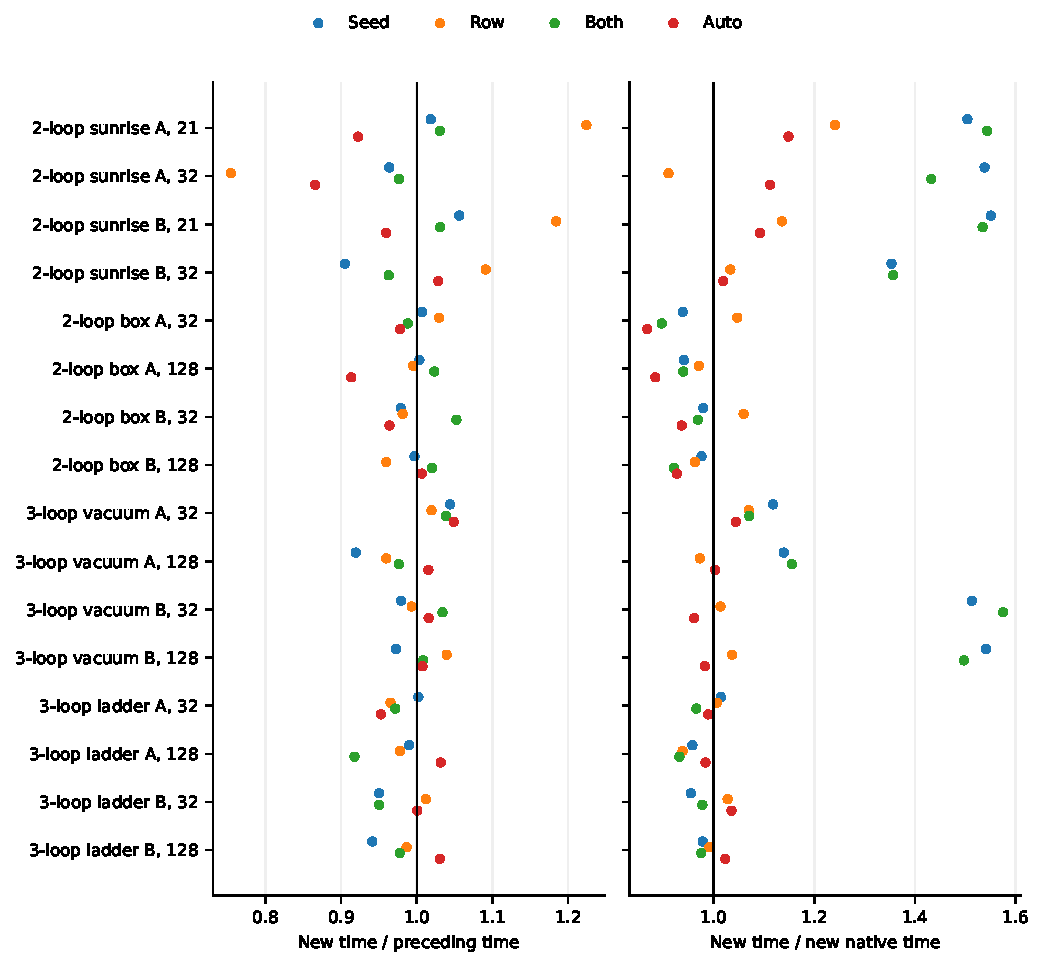
\includegraphics[width=\linewidth]{figures/shared_evaluation_times.pdf}
\caption{Complete-time ratios after sharing model calculations. The left panel
compares each method with its preceding implementation, and the right panel
compares it with the new native control. Every point uses the median of five
repetitions for one target batch. The tests keep model weights and algebraic
choices fixed, include unsuccessful attempts, and reuse the preceding eight
physical profiles.}
\label{fig:shared-evaluation}
\end{figure}

The production interface uses the shared calculations with the unchanged
validation-selected routing rule. Eight additional application checks supply
only the family, target indices and master indices to the reducer, then compare
its outputs independently with retained reference coefficients. All eight
checks pass. The original model checkpoints, preceding implementations and
negative comparisons remain available.

The operation counts are unchanged between implementations because the models
choose the same seeds and source rows. The saving comes from calculating these
choices with less repeated work. The comparison establishes measured costs for
the stated two- and three-loop inputs with fixed rational kinematics and
symbolic dimension $d$. A general gain across unrestricted higher-loop
families and a globally fastest reduction remain outside this evidence.
\clearpage
